% !TEX TS-program = pdflatex
% !TEX encoding = UTF-8 Unicode

% This is a simple template for a LaTeX document using the "article" class.
% See "book", "report", "letter" for other types of document.

%\usepackage{extsizes}

\documentclass[12pt]{article} % use larger type; default would be 10pt
%\documentclass[14pt]{extarticle} % use larger type; default would be 10pt

\usepackage[utf8]{inputenc} % set input encoding (not needed with XeLaTeX)

%%% Examples of Article customizations
% These packages are optional, depending whether you want the features they provide.
% See the LaTeX Companion or other references for full information.

%%% PAGE DIMENSIONS
\usepackage{geometry} % to change the page dimensions
\geometry{a4paper} % or letterpaper (US) or a5paper or....
%\geometry{margin=2in} % for example, change the margins to 2 inches all round
\geometry{left=2.0cm, right=2.0cm, top=3.5cm, bottom=4.5cm}
% \geometry{landscape} % set up the page for landscape
%   read geometry.pdf for detailed page layout information

\usepackage{graphicx} % support the \includegraphics command and options

% \usepackage[parfill]{parskip} % Activate to begin paragraphs with an empty line rather than an indent

%%% PACKAGES
\usepackage{booktabs} % for much better looking tables
\usepackage{array} % for better arrays (eg matrices) in maths
\usepackage{paralist} % very flexible & customisable lists (eg. enumerate/itemize, etc.)
\usepackage{verbatim} % adds environment for commenting out blocks of text & for better verbatim
\usepackage{subfig} % make it possible to include more than one captioned figure/table in a single float
% These packages are all incorporated in the memoir class to one degree or another...

%%% HEADERS & FOOTERS
\usepackage{fancyhdr} % This should be set AFTER setting up the page geometry
\pagestyle{fancy} % options: empty , plain , fancy
\renewcommand{\headrulewidth}{0pt} % customise the layout...
\lhead{}\chead{}\rhead{}
\lfoot{}\cfoot{\thepage}\rfoot{}

%%% SECTION TITLE APPEARANCE
%\usepackage{sectsty}
%\allsectionsfont{\sffamily\mdseries\upshape} % (See the fntguide.pdf for font help)
% (This matches ConTeXt defaults)

%%% BibTex packages (url for website references)
\usepackage[english]{babel}
\usepackage[round]{natbib}
% \usepackage{url}
% \usepackage{Biblatex}

%%% END Article customizations

%%% Change distance between bullet points
\usepackage{enumitem}
%\setlist{noitemsep}
\setlist{itemsep=0.15pt, topsep=6pt, partopsep=0pt}
%\setlist{nosep} % or \setlist{noitemsep} to leave space around whole list


%%% AMS math
\usepackage{amsmath}

% % % AMS symbols
\usepackage{amssymb}


%%% For coloneqq
\usepackage{mathtools}

\title{Collapsed Gibbs sampler}
%
\author{Stephen Coleman}

\begin{document} 
	\maketitle
	
	\section{Gibbs sampling}
	
	Consider Gibbs sampling of some vector of variables $\theta=(\theta_1,\ldots,\theta_p)$. Gibbs sampling works by iterating over each variable to be predicted, updating it based upon the current values of all the other variables and then repeating this a large number of times. Let $\theta^{(j)}=(\theta^{(j)}_1,\ldots,\theta^{(j)}_n)$ be the predicted values of $\theta$ in the $j^{th}$ iteration of Gibbs sampling. Our update for $\theta^{(j)}_i$ is conditioned on all the current values for the other variables - this means that the first $(i-1)$ variables have already been updated $j$ times, but the remaining $p - i$ variables are still based upon the $(j-1)^{th}$ iteration, i.e. our update probability is of the form:
	\[
	p\left(\theta^{(j)}_i | \theta^{(j)}_1,\ldots,\theta^{(j)}_{i-1},\theta^{(j-1)}_{i+1},\ldots, \theta^{(j - 1)}_p\right)
	\]
	Now, consider Gibbs sampling for a mixture of $K$ components for data $x=(x_1, \ldots, x_n)$, allocation variables $z=(z_1,\ldots,z_n)$, component parameters $\theta=(\theta_1,\ldots,\theta_K)$, and component weights $\pi=(\pi_1,\ldots,\pi_K)$. Let $x_{-i}$ indicate the vector $(x_1,\ldots,x_{i-1},x_{i+1},\ldots,x_n)$ and similarly for $z_{-i}$. Let our model be that described in figure \ref{fig:hierarchical_mode}.
	
	\begin{figure}[!htb]
		\centering
		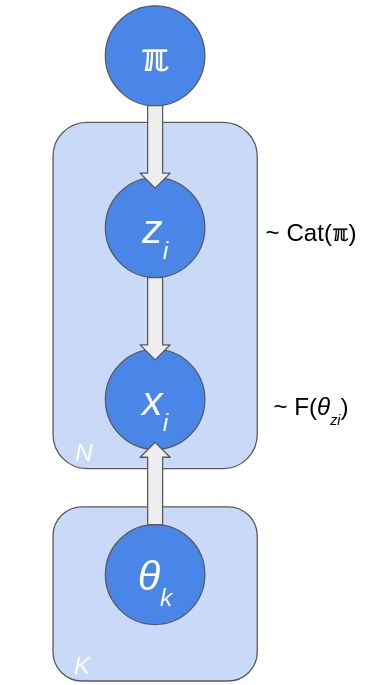
\includegraphics[scale=0.45]{./hierarchical_mixture_model.png}
		\caption{Hierarchical model for mixture model. Further hyperparameters can be included, but for our purposes of describing a collapsed Gibbs sampler this is sufficient.}
		\label{fig:hierarchical_mode}
	\end{figure}
	
	We are interested in the sampling of the $z$ variables. First recall that:
	\begin{eqnarray}
	p(A, B | C) &=& p(B | A, C) p (A | C) \\
	p(A|B, C) &=& \frac{p(A, B | C)}{P(B|C)} \\
	  &=& \frac{p(B | A, C) p (A | C)}{P(B|C)} \label{eqn:cond_prob} \\
	p(A | C) &=& \int_B p(A | B', C) p(B' | C) dB' \label{eqn:total_prob}
	\end{eqnarray}
	Now consider the sampling of $z_i$. As this can only hold a relatively small number of values we can consider the probability for each possible $k$. From our hierarchical model in figure \ref{fig:hierarchical_mode} and equations \ref{eqn:cond_prob}  and \ref{eqn:total_prob}:
	
	\begin{eqnarray}
		p(z_i = k | x, z_{-i}, \pi) &=& \frac{p(z_i = k | \pi, x_{-i}, z_{-i}, \pi) p(x_i | z, x_{-i}, \pi)}{p(x_i | x_{-i}, z_{-i}, \pi)} \label{eqn:placeholder} \\
		&\propto& p(z_i = k | \pi_k) \int_{\theta} p(x_i | \theta,  z, x_{-i}, \pi) p(\theta | z, x_{-i}, \pi) d \theta \\
		&=& \pi_k \int_{\theta} p(x_i | \theta) p(\theta | z, x_{-i}) d \theta \label{eqn:z_i_distn}
	\end{eqnarray}
	Note that $p(x_i | x_{-i}, z_{-i}, \pi)$ in the denominator is independent of $z_i$ and thus the same for all values of $k$.
	
	The integral in equation \ref{eqn:z_i_distn} is the posterior predictive distribution for $x_i$ given the other observations, $x_{-i}$. Thus, one may think of this as how well each component predicts $x_i$.
	
    An alternative way of describing this involves the ratio of marginal likelihoods. As we are component specific (given $z_i = k$), I drop the $z$ and $\pi$ from my conditional and assume we are referring only to the $x_j$ for which $z_j = k$.
    
    \begin{eqnarray}
    p(x_i | z, x_{-i}, \pi) &=& \frac{p(x | z)}{p(x_{-i} | z)} \\
      &=& \frac{\int_\theta p(x | \theta) p(\theta) d\theta}{\int_\theta p(x_{-i} | \theta) p(\theta) d\theta}
    \end{eqnarray}
    Therefore we can write the posterior predictive distribution as this ratio of marginal likelihoods:
    
    \begin{eqnarray}
    p(z_i = k | x, z_{-i}, \pi) \propto \pi_k \frac{p(x)}{p(x_{-i})}
    \end{eqnarray}
    Thus we can create a $K$-vector of probabilities for the allocation of $x_i$ to each component by finding the ratio of marginal likelihoods for each component including and excluding $x_i$, and multiplying these by the associated component weight, $\pi_k$. One can normalise these by dividing by the sum of the members of this vector due to the independence of the normalising constant from $z_i$.
	
	\section{Gaussian mixture models}
	
	In this section we derive the marginal likelihood for a component of the Gaussian mixture model assuming that the mean $\mu$ and the precision $\lambda$ are unknown. Before we can continue we state the associated probability density functions of the Normal and Gamma distributions:
	
	\begin{eqnarray}
	\mathcal{N}(x | \mu, \lambda^{-1}) &=& \sqrt{\frac{\lambda}{2\pi}} \exp \left(- \frac{\lambda}{2}(x - \mu) ^ 2\right) \\
	Ga(x | \alpha, \mathrm{rate }= \beta) &=& \frac{\beta^\alpha}{\Gamma(\alpha)} x ^{\alpha - 1} \exp(-\beta x)
	\end{eqnarray}
	
	\subsection{Likelihood}
	The model likelihood for $n$ observations is:
	
	\begin{eqnarray}
	p(x | \mu, \lambda) &=& \left(\frac{\lambda}{2\pi}\right)^{\frac{n}{2}}\exp\left(-\frac{\lambda}{2} \sum_{i=1}^n(x_i - \mu)^2 \right) \label{eqn:ngamma_likelihood_1}
	\end{eqnarray}
	Considering specifically the sum within the exponent here in equation \ref{eqn:ngamma_likelihood_1}, and letting $\bar{x}$ be the sample mean:
	\begin{eqnarray}
	\sum_{i=1}^n(x_i - \mu)^2 &=& \sum_{i=1}^n(x_i - \bar{x} + \bar{x} - \mu)^2 \\
	&=& \sum_{i=1}^n\left[(x_i - \bar{x})^2 + (\mu - \bar{x})^2 + 2(x_i \bar{x} - \bar{x}^2 - x_i \mu + \bar{x} \mu)\right] \\
	&=& n(\mu - \bar{x})^2 + \sum_{i=1}^n (x_i - \bar{x})^2
	\end{eqnarray}
	Substituting this back into equation \ref{eqn:ngamma_likelihood_1}, we have:
	\begin{eqnarray}
	p(x | \mu, \lambda) &=& \left(\frac{\lambda}{2\pi}\right)^{\frac{n}{2}}\exp\left(-\frac{\lambda}{2} \left[n(\mu - \bar{x})^2 + \sum_{i=1}^n (x_i - \bar{x})^2\right] \right) \label{eqn:likelihood}
	\end{eqnarray}
		
	\subsubsection{Prior}
	The conjugate prior for this model is the \emph{Normal-Gamma} distribution. This has the probability density function:
	
	\begin{eqnarray}
	NG(\mu, \lambda | \mu_0, \kappa_0, \alpha_0, \beta_0) &\coloneqq& \mathcal{N}(\mu | \mu_0, (\kappa_0 \lambda)^{-1})Ga(\lambda | \alpha_0, \beta_0) \\
	&=&  \sqrt{\frac{\kappa_0 \lambda}{2\pi}} \exp \left(- \frac{\kappa_0 \lambda}{2}(\mu - \mu_0) ^ 2\right) \\
	& & \hspace{3mm} \times \hspace{3mm} \frac{\beta_0 ^{\alpha_0}}{\Gamma(\alpha_0)} \lambda ^{\alpha_0 - 1} \exp(-\beta_0 \lambda) \\
	&=& \sqrt{\frac{\kappa_0}{2\pi}} \frac{\beta_0 ^ {\alpha_0}}{\Gamma(\alpha_0)} \\
	& & \hspace{3mm} \times \hspace{3mm}  \lambda^{\alpha_0 - \frac{1}{2}} \exp\left(-\frac{\lambda}{2}\left[\kappa_0 (\mu - \mu_0)^2 + 2 \beta_0\right]\right) \label{eqn:prior_pdf}
	\end{eqnarray}
	Here the normalising constant is:
	
	\begin{eqnarray}
	Z_0^{-1} = \sqrt{\frac{\kappa_0}{2\pi}} \frac{\beta_0 ^ {\alpha_0}}{\Gamma(\alpha_0)}
	\end{eqnarray}
	One can see that this function in equation \ref{eqn:prior_pdf} will naturally complement the likelihood described in equation \ref{eqn:likelihood}.
	
	\subsection{Posterior}
	From Bayes' theorem we have:
	
	\begin{eqnarray}
	p(\mu, \lambda | x) &\propto& p(x | \mu, \lambda) p(\mu, \lambda) \\
	&=& \left(\frac{\lambda}{2\pi}\right)^{\frac{n}{2}}\exp\left(-\frac{\lambda}{2} \left[n(\mu - \bar{x})^2 + \sum_{i=1}^n (x_i - \bar{x})^2\right] \right) \\
	&& \hspace{3mm} \times \hspace{3mm} \lambda^{\alpha_0 - \frac{1}{2}} \exp\left(-\frac{\lambda}{2}\left[\kappa_0 (\mu - \mu_0)^2 + 2 \beta_0\right]\right) \\
	&\propto&  \lambda^{\alpha_0 + \frac{n}{2} - \frac{1}{2}} \exp \left\{-\frac{\lambda}{2}\left[n(\mu - \bar{x})^2 + \kappa_0(\mu - \mu_0)^2 + \sum_{i=1}^n(x_i - \bar{x})^2 + 2\beta_0\right]\right\} \label{eqn:posterior_step_1}
	\end{eqnarray}
	We try and anticipate the parameters of our posterior. The following piece of logic might be slightly misleading. If one considers our prior as originating from previously observed data, we can consider the $\kappa_0$ parameter as the number of observations forming our prior and $\mu_0$ as the mean observed in our prior. In this case we would now expect that the observed mean, $\mu_n$, should correspond to a weighted average of combining the currently observed mean ($\bar{x}$), the number of observations in the current dataset ($n$) and these variables. Similarly, the ``total'' number of observations  between the prior data and the current data, $\kappa_n$, should be the sum of the number of samples in each, i.e.:
	
	\begin{eqnarray}
	\kappa_n &=& \kappa_0 + n \\
	\mu_n &=& \frac{\kappa_0 \mu_0 + n \bar{x}}{\kappa_0 + n}
	\end{eqnarray}
	If this is the case we would expect a term in the exponent:
	
	\begin{eqnarray}
	\kappa_n (\mu - \mu_n)^2 &=& (\kappa_0 + n)\left[\mu - \left(\frac{\kappa_0 \mu_0 + n \bar{x}}{\kappa_0 + n}\right)\right]^2 \\
	&=& (\kappa_0 + n) \left(\mu^2 - 2\mu(\kappa_0 \mu_0 + n \bar{x}) - \left(\frac{\kappa_0 \mu_0 + n \bar{x}}{\kappa_0 + n}\right)^2\right) %\\
	%&=& \kappa_0 \mu^2 + n\mu^2 - 2\mu (\kappa_0 + n) (\kappa_0 \mu_0 + n \bar{x}) - \frac{(\kappa_0\mu_0)^2 + 2n\kappa_0\mu_0 \bar{x} + (n\bar{x})^2}{\kappa_0 + n}
	\end{eqnarray}
	Returning to equation \ref{eqn:posterior_step_1} and considering the part of the exponent containing $\mu$:
	
	\begin{eqnarray}
	\kappa_0 (\mu - \mu_0) ^ 2 + n (\mu - \bar{x}) ^2 &=& \mu^2 (\kappa_0 + n) + n\bar{x}^2 + \kappa_0 \mu_0^2 -2n\mu\bar{x} -2 \kappa_0 \mu \mu_0 \\
	&=& (\kappa_0 + n) \left[\mu^2 + \frac{n\bar{x}^2}{\kappa_0 + n} + \frac{\kappa_0 \mu_0^2}{\kappa_0 + n} - 2 \mu \left(\frac{n\bar{x} + \kappa_0 \mu_0}{\kappa_0 + n}\right) \right] \label{eqn:posterior_exponent_expansion}
	\end{eqnarray}
	Notice that several of the desired terms are present, focusing on the components of this equation that do not fit our expected form:
	
	\begin{eqnarray}
	\frac{n\bar{x}^2}{\kappa_0 + n} + \frac{\kappa_0 \mu_0^2}{\kappa_0 + n} &=& \frac{n(\kappa_0 + n)\bar{x}^2 + \kappa_0(\kappa_0 + n)\mu_0^2}{(\kappa_0 + n)^2} \\
	&=& \frac{n^2 \bar{x}^2 + 2\kappa_0 n \mu_0 \bar{x} + \kappa_0^ 2 \mu_0 ^ 2}{(\kappa_0 + n)^2} 2 \frac{\kappa_0 n \bar{x}^2 + \kappa_0 n\mu_0^2 - 2\kappa_0 n \mu_0 \bar{x}}{(\kappa_0 + n)^2} \\
	\\
	&=& \left(\frac{n\bar{x} + \kappa_0 \mu_0}{\kappa_0 + n}\right)^2 + \frac{n\kappa_0\left(\bar{x} - \mu_0 \right)^2}{(\kappa_0 + n)^2}
	\end{eqnarray}
	Substituting this result into equation \ref{eqn:posterior_exponent_expansion} gives us:
	
	\begin{eqnarray}
	\kappa_0 (\mu - \mu_0) ^ 2 + n (\mu - \bar{x}) ^2 &=& (\kappa_0 + n) \left[\mu + \left(\frac{n\bar{x} + \kappa_0 \mu_0}{\kappa_0 + n}\right) \right]^2 + \frac{n\kappa_0\left(\bar{x} - \mu_0 \right)^2}{\kappa_0 + n}
	\end{eqnarray}
	Returning to equation \ref{eqn:posterior_step_1}:
	
	\begin{eqnarray}
	p(\mu, \lambda | x) &\propto& \lambda^{\alpha_0 + \frac{n}{2} - \frac{1}{2}} \exp \left\{-\frac{\lambda}{2}\left[
	(\kappa_0 + n) \left(\mu + \left(\frac{n\bar{x} + \kappa_0 \mu_0}{\kappa_0 + n}\right) \right)^2 + \frac{n\kappa_0\left(\bar{x} - \mu_0 \right)^2}{\kappa_0 + n} + \sum_{i=1}^n(x_i - \bar{x})^2 + 2\beta_0\right]\right\} \label{eqn:posterior}
	\end{eqnarray}
	This is the probability density function of a Normal-Gamma distribution.
	
	\begin{eqnarray}
	p(\mu, \lambda| x) &=& NG(\mu, \lambda | \mu_n, \kappa_n, \alpha_n, \beta_n) \\
	\mu_n &=& \frac{n\bar{x} + \kappa_0 \mu_0}{\kappa_0 + n} \\
	\kappa_n &=& \kappa_0 + n \\
	\alpha_n &=& \alpha_0 + \frac{n}{2} \\
	\beta_n &=& \beta_0 + \frac{1}{2}\sum_{i=1}^n(x_i - \bar{x})^2 + \frac{n\kappa_0\left(\bar{x} - \mu_0 \right)^2}{2(\kappa_0 + n)}
	\end{eqnarray}
	As this posterior distribution is $NG(\mu_n,\kappa_n, \alpha_n, \beta_n)$, we know that the associated normalising constant is:
	\begin{eqnarray}
	Z_n &=& \frac{\Gamma(\alpha_n)}{\beta_n^{\alpha_n}}\sqrt{\frac{2\pi}{\kappa_n}}.
	\end{eqnarray}
	
	\subsection{Marginal likelihood}
	Consider now the posterior but track the normalising constants (such as the $(2\pi)^{-n/2}$ in the likelihood). Denote the prior, likelihood and posterior less their normalising constants by $p'(\mu, \lambda)$, $p(x | \mu, \lambda)$ and $p'(\mu, \lambda | x)$ respectively:
	
	\begin{eqnarray}
	\frac{1}{Z_n} p'(\mu, \lambda | x) &=& \frac{1}{p(x)}\frac{1}{Z_0} p'(\mu, \lambda)\left(\frac{1}{2\pi}\right)^{\frac{n}{2}} p'(x | \mu, \lambda)
	\end{eqnarray}
	We know that the product of the unnormalised prior and the unnormalised likelihood give the right hand side of equation \ref{eqn:posterior}, and that this is our unnormalised posterior, $p'(\mu, \lambda | x)$. Thus:
	
	\begin{eqnarray}
	\frac{1}{Z_n} p'(\mu, \lambda | x) &=& \frac{1}{p(x)}\frac{1}{Z_0} \left(\frac{1}{2\pi}\right)^{\frac{n}{2}} p'(\mu, \lambda | x) \\
	\implies p(x) &=& \frac{Z_n}{Z_0}(2\pi)^{-\frac{n}{2}} 
	\end{eqnarray}
	Thus our marginal likelihood is the ratio of the posterior normalising constants to the product of those of the likelihood and prior. Expanding this we finally have:
	
	\begin{eqnarray}
	p(x) &=& \frac{\Gamma(\alpha_n)}{\beta_n^{\alpha_n}} \sqrt{\frac{2\pi}{\kappa_n}} \frac{\beta_0^{\alpha_0}}{\Gamma(\alpha_0)} \sqrt{\frac{\kappa_0}{2\pi}} (2\pi)^{-\frac{n}{2}} \\
	&=& \frac{\Gamma(\alpha_n)}{\Gamma(\alpha_0)}\frac{\beta_0^{\alpha_0}}{\beta_n^{\alpha_n}} \sqrt{\frac{\kappa_0}{\kappa_n}}(2\pi)^{-\frac{n}{2}}
	\end{eqnarray}

	
\end{document}